\chapter{Практическая часть}

В этом разделе будет описано задание и приведено его решение.

\section{Задание:}
Составить программу -- базу знаний, с помощью которой можно определить, например, множество студентов, обучающихся в одном ВУЗе. Студент может одновременно обучаться в нескольких ВУЗах. Привести примеры возможных вариантов вопросов и варианты ответов (не менее 3-х). Описать порядок формирования ответа.

На листинге ниже представлен текст разработанной программы.

\lstset{language=python}
\begin{lstlisting}[caption=Текст программы]
domains
   name, university, city = symbol.

predicates
  college(university, city).
  study(name, university).

  studying_in(name, city).

clauses
  college(msu, moscow).
  college(bmstu, moscow).
  college(mit, boston).
  college(nsu, novosibirsk).
  college(itmo, piter).

  study(tolya, msu).
  study(kolya, itmo).
  study(olya, bmstu).
  study(eric, mit).
  study(sasha, bmstu).
  study(misha, nsu).
  study(misha, College) :- study(eric, College).
  study(dasha, itmo).
  study(olya, msu).

  studying_in(Name, City) :- study(Name, College),
                                college(College, City).
goal
  %study(sasha, bmstu).
  %study(olya, College).
  %study(Name, msu).
  %college(nsu, _).
  studying_in(Person, piter).
\end{lstlisting}

\section{Примеры работы:}
\begin{enumerate}
    \item sasha учится в bmstu?
\begin{figure}[H]
    \centering
    
\includegraphics[scale=1.5]{data/image/1.png}
    \caption{study(sasha, bmstu).}
\end{figure}

    \item в каких университетах учится olya?
\begin{figure}[H]
    \centering
    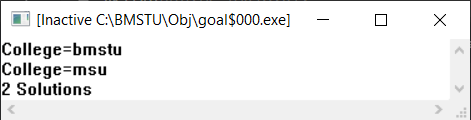
\includegraphics[scale=1.5]{data/image/2.png}
    \caption{study(olya, College).}
\end{figure}
    \item кто учится в msu?
\begin{figure}[H]
    \centering
    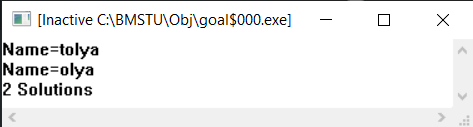
\includegraphics[scale=1.5]{data/image/3.png}
    \caption{study(Name, msu).}
\end{figure}
    \item nsu - университет?
\begin{figure}[H]
    \centering
    
\includegraphics[scale=1.5]{data/image/4.png}
    \caption{college(nsu, \_).}
\end{figure}
    \item кто учится в piter?
\begin{figure}[H]
    \centering
    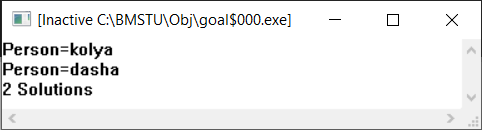
\includegraphics[scale=1.5]{data/image/5.png}
    \caption{studying\_in(Person, piter).}
\end{figure}


\end{enumerate}
